Table~\ref{tab:datasets} summarizes the data samples used in the current analysis, 
the channels in which they are used, and the approximate luminosity as reported in 
the particular {\tt JSON} file used in each analysis.  
Tables~\ref{tab:SigMC}--\ref{tab:ttbarMC} summarize the simulated samples and their 
equivalent luminosities.  {\tt Fall11} samples are used consistently for all the analysis steps.
 Appropriate pile-up reweighting is 
applied when comparing to data, in order to represent the true primary vertex 
distribution in the different run ranges.  An example of the effect of reweighting
is shown in Fig.~\ref{fig:PVreweight}, which shows the distribution of the number of
primary vertices in data and reweight {\tt Fall11} simulation for a sample of Z$(\mu\mu)$ +jet events
selected as described in Sec.~\ref{sec:Vselection}.  The samples were analyzed with CMSSW 
version 4.2.x and processed through the standard PAT configuration.

\begin{figure}[htbp]
\begin{center}
\subfigure{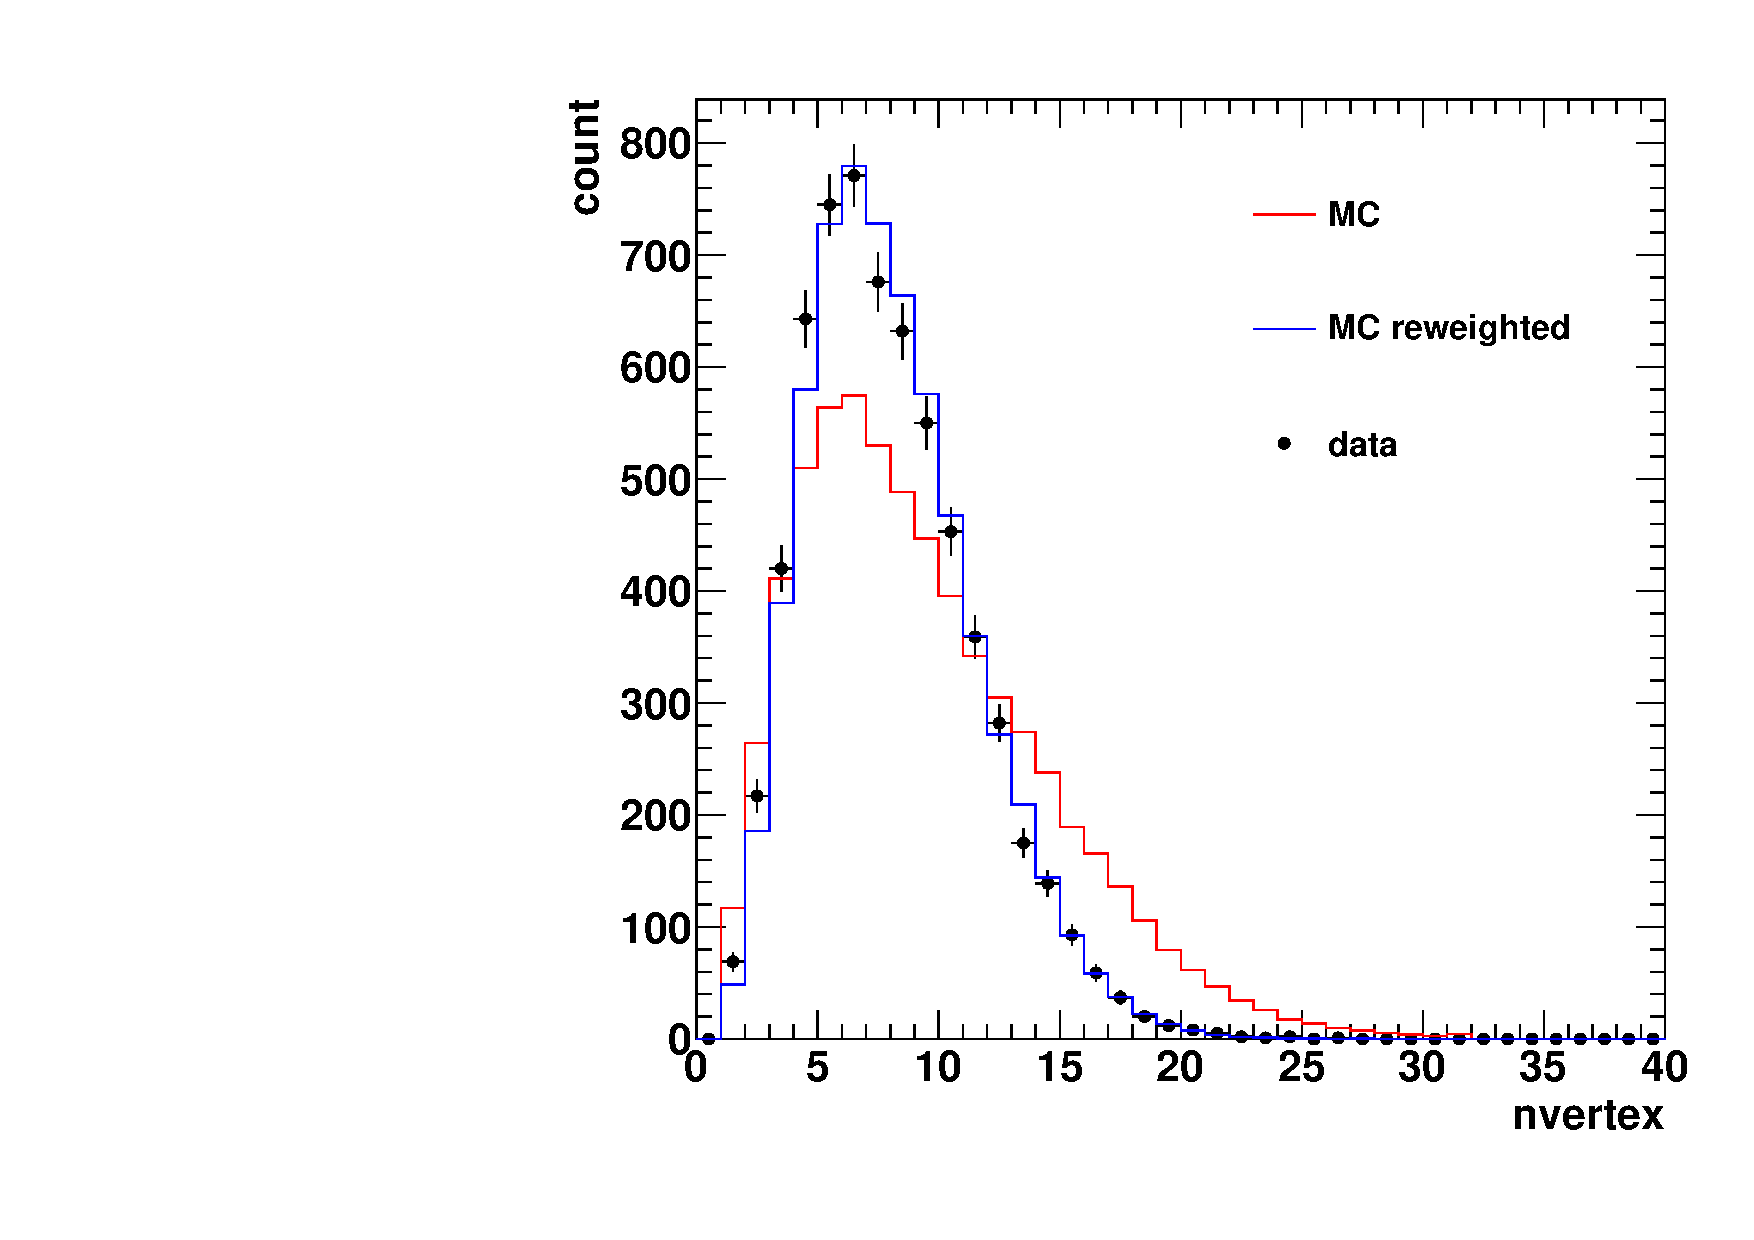
\includegraphics[width=0.49\textwidth]{figs/n_vertices.pdf}}
%    \includegraphics[width=0.48\textwidth]{figures/WmnH-ttbar-nPV-lin}
%    \includegraphics[width=0.48\textwidth]{figures/WmnH-ttbar-nPV-log}
    \caption{Distribution of the number of reconstructed primary vertices in
    data compared to simulation in a sample of Z$(\mu\mu)$+jet events   
    selected as discussed in Sec.~\ref{sec:Vselection} }
    \label{fig:PVreweight}
  \end{center}
\end{figure}

\begin{table}[tbp]
\caption{List of 2011 data samples used for this analysis.  The sum includes approximately
$5. \fbinv$ across all modes.}
\label{tab:datasets}
\begin{center}
\begin{tabular}{ccc} \hline\hline
        Mode                    & Dataset                                           & $\cal L$ (\fbinv) \\\hline
W$(\Pgm\cPgn)$, Z$(\Pgm\Pgm)$ & {\tt /SingleMu/Run2011/May10ReReco}	            & $0.2110$ \\
                                & {\tt /SingleMu/Run2011A/Aug05ReReco}	            & $0.3953$ \\
                                & {\tt /SingleMu/Run2011A/PromptRecoV4}	            & $0.9547$ \\
                                & {\tt /SingleMu/Run2011A/PromptRecoV6}	            & $0.7067$ \\
                                & {\tt /SingleMu/Run2011B/PromptRecoV1}	            & $2.707$ \\
\hline
				& Total Lumi                                        & $4.9748$ \\\hline\hline
W$(\Pe\cPgn)$                  & {\tt /SingleElectron/Run2011/May10ReReco}         &  $0.2156$ \\
                                & {\tt /ElectronHad/Run2011A/Aug05ReReco}           & $0.3953$ \\
                                & {\tt /ElectronHad/Run2011A/PromptRecoV4}          & $0.9553$ \\
                                & {\tt /ElectronHad/Run2011A/PromptRecoV6}          & $0.7067$ \\
                                & {\tt /ElectronHad/Run2011B/PromptRecoV1}          & $2.709$ \\
\hline
				& Total Lumi                                        & $4.6754$ \\\hline\hline
Z$(\Pe\Pe)$                    & {\tt /DoubleElectron/Run2011/May10ReReco}	    & $0.2155$ \\
                                & {\tt /DoubleElectron/Run2011A/Aug05ReReco} 	    & $0.3953$ \\
                                & {\tt /DoubleElectron/Run2011A/PromptRecoV4}       & $0.9553$ \\
                                & {\tt /DoubleElectron/Run2011A/PromptRecoV6}       & $0.7067$ \\
                                & {\tt /DoubleElectron/Run2011B/PromptRecoV1}       & $2.709$ \\
\hline
				& Total Lumi                                        & $4.9818$ \\\hline\hline
\hline\hline
\end{tabular}
\end{center}
\end{table}

\begin{table}[tbp]
\caption{List of diboson {\tt Fall11} Monte Carlo samples used in this version of the note.}
\label{tab:SigMC}
\begin{center}
\begin{tabular}{ccc} \hline\hline
        Mode          & Dataset				       & $\cal L\,(\fbinv)$ \\ \hline
{\small ZZ		      } & {\small  {\tt /ZZtoAnything\_TuneZ2\_7TeV-pythia6-tauola  }}	     & {\small $  675.912 $ } \\
{\small WW		      } & {\small  {\tt /WWtoAnything\_TuneZ2\_7TeV-pythia6-tauola  }}	     & {\small $  98.38 $ } \\
{\small WZ		      } & {\small  {\tt /WZtoAnything\_TuneZ2\_7TeV-pythia6-tauola  }}	     & {\small $  234.35$ } \\
\hline\hline
\end{tabular}
\end{center}
\end{table}

\begin{table}[tbp]
\caption{List of V+jets {\tt Fall11} Monte Carlo samples used in this version of the note.}
\label{tab:VjetsMC}
\begin{center}
\begin{tabular}{ccc} \hline\hline
% update of lumi values for Vjets
        Mode          & Dataset				       & $\cal L\,(\fbinv)$ \\ \hline
%{\tiny W+jets  			} & {\tiny  {\tt /WjetsToLNu\_TuneZ2\_7TeV-madgraph-tauola }}	           & {\tiny $  2.598   $ } \\
{\small W+jets $(\pt >100\GeV)$   	} & {\small  {\tt /WjetsToLNu\_pt100\_7TeV-madgraph-tauola }}	           & {\small $  32.02 $ } \\
{\small W+jets $(\pt >100\GeV)$          } & {\small {\tt /WjetsToLNu\_pt100\_7TeV-herwigpp }}              & {\small $  86.99 $ } \\
%{/tiny Z$\to\ell\ell(M_{\ell\ell}>50)$ } & {\tiny  {\tt /DYJetsToLL\_TuneZ2\_M-50\_7TeV-madgraph-tauola }} & {\tiny $  11.51   $ } \\
{\small Z$\to\ell\ell(\pt > 100\GeV)$ }   & {\small  {\tt /DYJetsToLL\_pt100\_7TeV-madgraph-tauola }}        & {\small $  33.8 $ } \\
{\small Z$\to\cPgn\ell(\pt > 100\GeV)$ }  & {\small  {\tt /DYJetsToLL\_Pt-100\_7TeV-herwigpp }}             & {\small $  81.8 $ } \\
\hline\hline
\end{tabular}
\end{center}
\end{table}

\begin{table}[tbp]
\caption{List of \ttbar\ and single top, and QCD {\tt Fall11} samples used in this analysis.
}
\label{tab:ttbarMC}
\begin{center}
\begin{tabular}{ccc} \hline\hline
        Mode          & Dataset				       & $\cal L\,(\fbinv)$ \\ \hline
{\tiny \ttbar\ 	 } & {\tiny {\tt /TTJets\_TuneZ2\_7TeV-madgraph-tauola/11-PU\_S6\_START42\_V14-v2/AODSIM             }}         & {\tiny $360.$ } \\
{\tiny Single Top (tW)	 } & {\tiny {\tt /T\_TuneZ2\_tW-channel-DR\_7TeV-powheg-tauola/11-PU\_S6\_START42B\_V14-v1/AODSIM     }} & {\tiny $103.5$ } \\
                           & {\tiny {\tt /Tbar\_TuneZ2\_tW-channel-DR\_7TeV-powheg-tauola/11-PU\_S6\_START42B\_V14-v1/AODSIM  }} & {\tiny $102.9$ } \\
{\tiny Single Top (t-ch)} & {\tiny {\tt /T\_TuneZ2\_t-channel\_7TeV-powheg-tauola/11-PU\_S6\_START42B\_V14-v1/AODSIM         }}  & {\tiny $93.0$  } \\
                           & {\tiny {\tt /Tbar\_TuneZ2\_t-channel\_7TeV-powheg-tauola/11-PU\_S6\_START42B\_V14-v1/AODSIM      }} & {\tiny $85.9$  } \\
{\tiny Single Top (s-ch)} & {\tiny {\tt /T\_TuneZ2\_s-channel\_7TeV-powheg-tauola/11-PU\_S6\_START42B\_V14-v1/AODSIM         }}  & {\tiny $81.5$  } \\
                           & {\tiny {\tt /Tbar\_TuneZ2\_s-channel\_7TeV-powheg-tauola/11-PU\_S6\_START42B\_V14-v1/AODSIM      }} & {\tiny $95.8$  } \\
%{\tiny QCD(muon)	 } & {\tiny {\tt /QCD\_Pt-20\_MuEnrichedPt-15\_TuneZ2\_7TeV-pythia6/11-PU\_S6\_START42B\_V14-v2/AODSIM}} & {\tiny $0.296$ } \\
%{\tiny QCD(electron)	 } & {\tiny {\tt /QCD\_Pt-80to120\_TuneZ2\_7TeV\_pythia6/11-PU\_S\_START42\_V11-v1/AODSIM  }}	      & {\tiny $0.008$ } \\
%{\tiny QCD(electron)	 } & {\tiny {\tt /QCD\_Pt-120to170\_TuneZ2\_7TeV\_pythia6/11-PU\_S\_START42\_V11-v1/AODSIM }}	      & {\tiny $0.053$ } \\
%{\tiny QCD(electron)	 } & {\tiny {\tt /QCD\_Pt-170to300\_TuneZ2\_7TeV\_pythia6/11-PU\_S\_START42\_V11-v1/AODSIM }}	      & {\tiny $0.256$ } \\
%{\tiny QCD(electron)	 } & {\tiny {\tt /QCD\_Pt-300to470\_TuneZ2\_7TeV\_pythia6/11-PU\_S\_START42\_V11-v1/AODSIM }}	      & {\tiny $5.500$ } \\
%{\tiny QCD(electron)	 } & {\tiny {\tt /QCD\_Pt-470to600\_TuneZ2\_7TeV\_pythia6/11-PU\_S\_START42\_V11-v1/AODSIM }}	      & {\tiny $56.8$  } \\
\hline\hline
\end{tabular}
\end{center}
\end{table}

